\documentclass[11pt]{article}
\usepackage[margin=1.15in]{geometry}
\usepackage{amsmath,amssymb,amsthm}
\usepackage{booktabs}
\usepackage{tabularx}
\usepackage{tikz}
\usetikzlibrary{positioning}
\usepackage{microtype}
\usepackage{enumitem}
\usepackage[colorlinks=true,linkcolor=black,citecolor=black,urlcolor=black]{hyperref}

\theoremstyle{definition}
\newtheorem{definition}{Definition}
\theoremstyle{remark}
\newtheorem{remark}{Remark}

\newcommand{\norm}[1]{\lVert #1\rVert}
\newcommand{\XtX}{X^{\!\top}\!X}

\title{The Unequal Error:\\
Precision, Propagation, and the Architecture of Consequence}
\author{Flyxion\\\small Independent Researcher}
\date{September 2026}

\begin{document}
\maketitle

\begin{abstract}
\noindent
Ding et al.\ (\textit{Nature Communications}, 2026) run singular value decomposition on analog memristor hardware whose stored numbers are imprecise and whose readouts fluctuate. Their selective representation enhanced architecture (SREA) does not raise precision everywhere. It assigns precision to the places where an error would do the most damage: the high-order parts of the data matrix, and the inputs to previously computed singular vectors whose errors are amplified during deflation. The engineering result is a large gain in accuracy and a near halving of energy at a few percent of extra area. The conceptual result is that the paper treats error according to its consequence and not according to its size. This essay states that principle in terms of error propagation, derives a first-order sketch of why the two failure modes of power iteration with deflation differ, formulates precision allocation as a budget problem that the paper does not itself pose, and reads the paper's incremental-learning results as a case in which a persisting decomposition is kept available for revision. The paper's claims are separated throughout from the abstractions built on them, and the limits of the evidence are listed at the end.
\end{abstract}

\section{Two accountings of error}

Ordinary practice measures an error by its size. A perturbation of one part in a thousand is a small error and a perturbation of one part in ten is a large one, and a precision requirement is a bound on that size, applied to every stored number alike. Hardware whose stored values are physically noisy makes the uniform requirement expensive, because the cost of holding a number to a given tolerance rises steeply as the tolerance tightens.

The memristive singular value decomposition (MSVD) of Ding et al.\ is built on a different accounting. The decomposition is computed iteratively, one singular vector at a time, and an error made early is not merely present in the result. It is carried into later operations that transform it. The paper's architecture assigns different precisions to different parts of the computation, and it does so because the parts differ in what their errors can later damage.

This essay follows that difference. The claim to be defended is modest to state and broad in application: \emph{an error is characterized not only by how wrong it is, but by where it can go.} Error magnitude is a property of a perturbation. Error consequence is a property of a perturbation together with the computation that will subsequently act on it.

\section{The computation and its two failure geometries}

Let $X\in\mathbb{R}^{M\times N}$ have singular value decomposition $X=USV^{\top}$, with singular values $s_1>s_2>\cdots>0$ and right singular vectors (RSVs) $v_i$ forming the columns of $V$. The paper extracts the vectors sequentially by power iteration with deflation. For the $i$-th vector, the iterate is updated as
\begin{equation}
  \tilde v \;\leftarrow\; \operatorname{norm}\!\Big(\big(\XtX - V_{i-1}S_{i-1}^{2}V_{i-1}^{\top}\big)\tilde v\Big),
  \label{eq:deflation}
\end{equation}
where $V_{i-1}$ and $S_{i-1}$ hold the RSVs and singular values already solved. The first term is one step of power iteration on the data matrix. The second removes the components belonging to earlier vectors, which is the deflation. On the memristor hardware the data matrix and the previously solved RSVs are stored on two crossbar arrays and both multiplications are executed in place, with the scaling by $S^2$, the subtraction, and the normalization handled by digital peripherals.

The paper identifies two failures, and their separation is the first fact that matters.

\emph{Numerical drift.} Conductance fluctuations in the memristors perturb every multiplication by the data matrix. The errors accumulate as the iteration proceeds, producing unstable convergence and imprecise output for the vector being solved.

\emph{Component residual.} The stored RSVs are imperfect copies of the true vectors, because of mapping deviations when they are written, and because the coefficients fed to them are quantized. During deflation the subtraction therefore removes the earlier component only approximately. A remainder is left behind, and the paper notes that a substantial remainder can influence or even replace later target singular vectors.

The two are different in origin and in what they threaten. Drift damages the vector currently being computed. A residual damages vectors that have not yet been computed, using a defect in vectors that were computed earlier. Figure~\ref{fig:chain} shows the dependency that makes the second failure possible: every solved vector is consumed by every later deflation.

\begin{figure}[t]
\centering
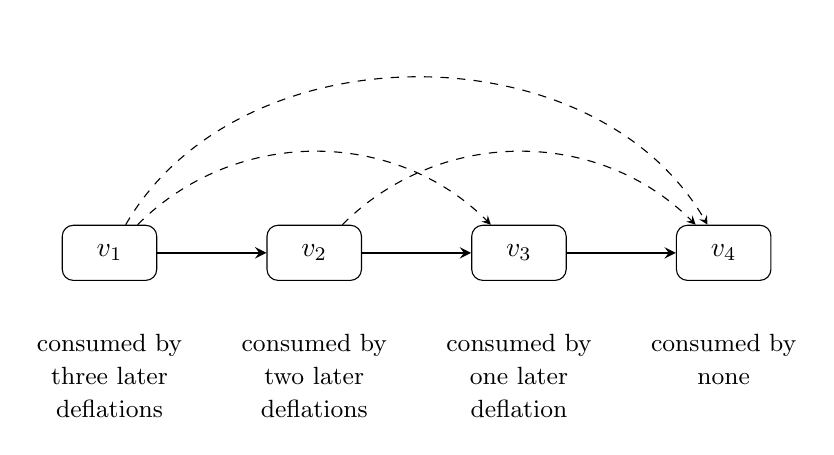
\begin{tikzpicture}[>=stealth,node distance=2.2cm]
  \foreach \i/\x in {1/0,2/2.6,3/5.2,4/7.8} {
    \node[draw,rounded corners,minimum width=1.2cm,minimum height=0.7cm] (v\i) at (\x,0) {$v_{\i}$};
  }
  \draw[->,thick] (v1) -- (v2);
  \draw[->,thick] (v2) -- (v3);
  \draw[->,thick] (v3) -- (v4);
  \draw[->,dashed] (v1) to[bend left=45] (v3);
  \draw[->,dashed] (v1) to[bend left=60] (v4);
  \draw[->,dashed] (v2) to[bend left=45] (v4);
  \node[below=0.55cm of v1,align=center] {\small consumed by\\\small three later\\\small deflations};
  \node[below=0.55cm of v2,align=center] {\small consumed by\\\small two later\\\small deflations};
  \node[below=0.55cm of v3,align=center] {\small consumed by\\\small one later\\\small deflation};
  \node[below=0.55cm of v4,align=center] {\small consumed by\\\small none};
\end{tikzpicture}
\caption{Solved vectors are stored and consumed. Solid arrows: extraction order. Dashed arrows: deflation dependencies. The number of downstream consumers of a stored vector decreases with its rank, so a defect in $v_1$ has more places to go than a defect in $v_3$.}
\label{fig:chain}
\end{figure}

\section{What the architecture does}

SREA has two components, one for each failure.

\emph{Dual-precision mapping (DPM)} addresses drift in the data matrix. Each stored number is split into a high-order part and a low-order part. For an 8-bit number, the paper's example puts the two high-order bits on a low-resolution array, meaning one in which each device holds one of only a few well-separated conductance levels, and the six low-order bits on a high-resolution array. The stated rationale is that a high-order bit carries a large positional weight, so a deviation there is multiplied by that weight, and it is therefore given the physically robust representation. The low-order bits carry small weights and receive the fine resolution that preserves numerical detail. The multiplication is recombined by a bit shift, $X\cdot Y=(X_hY)\ll l+X_lY$. The paper contrasts this with uniform bit slicing, where every position is treated alike.

\emph{Vector processing refinement (VPR)} addresses the residual. The inputs to the stored RSV array are scaled by the squared singular values, so they span a wide dynamic range, and quantization errors on them would be magnified in the subsequent multiplication. VPR encodes exactly these inputs with more bits than the standard system precision (12 bits within an 8-bit system, in the paper's example), and stores each solved RSV several times on the array, summing the replicas' outputs and averaging them to suppress device variation. The paper stresses that the extra precision and redundancy apply only to these inputs and to the small-sized singular vectors, not to the whole computation, and gives that as the reason overhead stays low.

The measured device noise shows why the split is sensible. The chip's mapping deviation has a standard deviation of $0.27\,\mu$S and the read fluctuation $0.21\,\mu$S, on devices programmed over roughly a 0 to 30\,$\mu$S range. If 32 levels are spread evenly over that range, adjacent levels are about $1\,\mu$S apart, so the noise is a substantial fraction of the level spacing. A device that holds only four levels over the same range has spacing near $10\,\mu$S and the same noise is small beside it. The precise allocations are in the paper's supplementary configurations and the arithmetic here is illustrative, but it displays the mechanism: putting the heavily weighted bits on coarse, well-separated states buys error immunity exactly where an error would be multiplied most.

\section{Propagation}

The formal content of the principle can be stated without reference to memristors. Let a computation be a sequence of maps $x_{t+1}=F_t(x_t)$. A perturbation $\delta x_t$ introduced at stage $t$ has downstream effect, to first order,
\begin{equation}
  \delta x_T \;\approx\; J_{T-1}J_{T-2}\cdots J_t\,\delta x_t,
  \label{eq:jacobian}
\end{equation}
where $J_s$ is the Jacobian of $F_s$. Two perturbations of equal norm need not have equal consequence, because the product of Jacobians can stretch one direction and shrink another:
\[
  \norm{\delta x^{(a)}_t}=\norm{\delta x^{(b)}_t}
  \quad\not\Rightarrow\quad
  \norm{\delta x^{(a)}_T}=\norm{\delta x^{(b)}_T}.
\]
This is the general fact. The SVD iteration supplies concrete instances of it, and each can be worked out to first order from Equation~\eqref{eq:deflation}. The following are derivations from standard perturbation reasoning and not claims made by the paper.

\subsection{Errors in the iterate wash out. Errors in the operator do not.}

Near convergence to $v_i$, the map $\tilde v\mapsto\operatorname{norm}(A_i\tilde v)$, with $A_i$ the deflated operator, has a Jacobian whose eigenvalues on directions orthogonal to $v_i$ are $s_k^2/s_i^2$ for $k>i$, all less than one. A perturbation of the iterate is therefore contracted at each step, at a rate set by the ratio $\rho=s_{i+1}^2/s_i^2$. This is the same ratio that governs convergence in the paper's Equation~2. A perturbation that instead sits in the operator, meaning an error in the stored matrix or in a stored vector, shifts the fixed point of the iteration. It is not contracted. It is reapplied on every step.

The consequence is that the errors worth protecting are those in the persistent, stored objects, which are the data matrix and the solved RSVs, and not those in the iterate. That is where SREA puts its structure.

Fresh noise added to the iterate at every step, as read fluctuation does, is not entirely harmless. Modeling the deviation as $e_{t+1}=\rho\,e_t+n_t$ with independent noise $n_t$ of variance $\sigma^2$ gives a steady-state variance of $\sigma^2/(1-\rho^2)$. A small spectral gap, with $\rho$ near one, therefore amplifies read noise, and does so in addition to slowing convergence. The heuristic points the same way as the paper's finding that the number of iterations grows roughly linearly with the logarithm of the normalized singular value gap, though that finding concerns convergence and not steady-state noise.

\subsection{Deflation residuals are amplified by the earlier singular value.}

Suppose a stored vector is $\hat v_j=v_j+\delta_j$. The deflated operator then differs from the exact one by
\[
  E \;\approx\; -\,s_j^{2}\big(v_j\delta_j^{\top}+\delta_j v_j^{\top}\big),
  \qquad \norm{E}\approx 2\,s_j^{2}\norm{\delta_j^{\perp}},
\]
where $\delta_j^{\perp}$ is the part of $\delta_j$ orthogonal to $v_j$. A Davis--Kahan style first-order bound then limits the resulting angular error in the extracted vector $v_i$ by
\begin{equation}
  \theta_i \;\lesssim\; \frac{\norm{E}}{s_i^{2}-s_{i+1}^{2}}
  \;\approx\; \Gamma_{j\to i}\,\norm{\delta_j^{\perp}},
  \qquad
  \Gamma_{j\to i} \;=\; \frac{2\,s_j^{2}}{s_i^{2}-s_{i+1}^{2}}.
  \label{eq:gamma}
\end{equation}
Three things follow. The amplification grows with $s_j^2$, so a defect in an early vector, with its large singular value, weighs more than the same defect in a later one. It grows as the gap $s_i^2-s_{i+1}^2$ of the target shrinks, so targets in a crowded part of the spectrum are the most fragile. And it applies once for each later $i$, so the total exposure of a stored vector is a sum over its downstream consumers, which is the count shown in Figure~\ref{fig:chain}. The paper's observation that the inputs to the RSV array are scaled by the square of the solved singular values is the hardware face of the $s_j^2$ factor in Equation~\eqref{eq:gamma}, and its supplementary treatment of resolution limits through Wedin's perturbation bound is the same kind of statement about gaps.

These derivations show that ``two identical errors'' have unequal consequences in this system in at least three independent ways: by whether they sit in the iterate or the operator, by the rank of the vector they are attached to, and by the spectral gap of the target that will consume them.

\section{Consequence and a precision budget}

The paper describes a design and demonstrates its effect. It does not state an optimization problem. The following formalization is the essay's own, offered to make the principle explicit and to separate it from the specific design.

Index the stored components by $c$, which may be a bit plane of the data matrix, an RSV input, or a replica. Let $\epsilon_c(p_c)$ be the expected error at precision setting $p_c$, and let $\mathcal{T}(c)$ be the set of downstream targets that consume $c$. Each target $i$ has a representational weight $w_i$, for example its share of the reconstructed energy, $s_i^2/\sum_k s_k^2$, and $\Gamma_{c\to i}$ is the propagation gain from $c$ to $i$ as in Equation~\eqref{eq:gamma}. Define the consequence of an error in $c$ as
\begin{equation}
  \mathcal{C}_c(p_c) \;=\; \epsilon_c(p_c)\sum_{i\in\mathcal{T}(c)} w_i\,\Gamma_{c\to i}.
  \label{eq:consequence}
\end{equation}
The three importances discussed informally in connection with the paper enter separately. The factor $w_i$ is \emph{representational importance}, how much of the result a target carries. The factor $\Gamma_{c\to i}$ is \emph{propagational importance}, how strongly an error in $c$ is amplified on its way to that target. The size of the set $\mathcal{T}(c)$ is \emph{dependency centrality}, how many operations consume the component. A precision allocation then solves
\begin{equation}
  \min_{\{p_c\}}\;\sum_c \mathcal{C}_c(p_c)
  \qquad\text{subject to}\qquad
  \sum_c K_c(p_c)\;\le\; B,
  \label{eq:budget}
\end{equation}
with $K_c$ the hardware cost of precision $p_c$ and $B$ the budget. For differentiable convex $\epsilon_c$ and $K_c$, the optimum equalizes marginal consequence reduction per unit cost across components,
\[
  \frac{-\,\partial\mathcal{C}_c/\partial p_c}{\partial K_c/\partial p_c} \;=\; \mu \quad\text{for every }c,
\]
where $\mu$ is the multiplier of the budget constraint. The optimal allocation is not equal precision. It is equal marginal return, which puts more precision where the sum in Equation~\eqref{eq:consequence} is large and less where it is small.

\begin{remark}
SREA is qualitatively of this form. It protects the components with large positional weight, and the components that are inputs to stored vectors scaled by large singular values, and it leaves the rest at baseline. This essay makes no claim that SREA solves Equation~\eqref{eq:budget}. The paper chooses its configurations per task (the supplementary tables give, for example, a two-bit and five-bit split for the small IRIS matrix and a three-bit and five-bit split for the gesture task) and reports a precision-cost balance, not an optimum.
\end{remark}

The formulation also explains why representational importance alone would mislead. The singular values order the components of the result by how much of the data they represent, $s_1\ge s_2\ge\cdots$. A rule that protected components in that order would protect $v_1$ most and the tail least. Equation~\eqref{eq:gamma} agrees about the head, because $s_1^2$ is the largest amplification. But the rule that protects by size would also treat every bit plane of the data matrix alike, and would miss that a plane's importance is set by its positional weight, and would miss that the least significant stored vectors matter a great deal less than the first ones only because they have fewer consumers, not because they represent less. Representation and propagation coincide at the head of the spectrum and separate elsewhere.

\section{What the paper shows}

The empirical results support the qualitative claim that the two failures are distinct and that treating them separately pays.

The main test uses the IRIS matrix, which is $150\times4$. Averaged over 20 runs, MSVD with SREA reduces the normalized error of the singular values by factors of 1.4, 11, 13, and 3.2 for $s_1$ through $s_4$, so that the best case is a $13\times$ improvement, and the standard deviation of RSV element error falls from $0.415$ to $0.192$. The gain is not uniform across ranks, and the smallest gain is at $s_1$. That is what the analysis above predicts: the first vector has no earlier vectors to be deflated against, so it can suffer drift but not residual. The paper does not explain the smaller gain at $s_4$ relative to $s_2$ and $s_3$.

The ablation separates the two components. Dual-precision mapping alone reduces singular value error by up to $8.0\times$ and vector processing refinement alone by up to $3.4\times$. The paper's reconstruction-error landscapes tell the same story in geometric terms. With DPM alone, each individual iteration has a steeper landscape but the system cannot maintain consistent convergence paths across the third and fourth ranks, because of interference from deflation residuals. With VPR alone, deflation is more thorough but numerical drift flattens the landscape and makes iterations inefficient at higher ranks. Only the combination produces effective trajectories. Table~\ref{tab:failures} sets the correspondence out.

\begin{table}[t]
\centering
\small
\begin{tabularx}{\textwidth}{@{}p{2.3cm}XXX@{}}
\toprule
Failure & Where the error lives & Why it is amplified & Remedy and ablation effect \\
\midrule
Numerical drift & Data matrix entries and read noise during the iteration for the current vector & High-order bits carry large positional weights; noise is reapplied every step & DPM: robust coarse states for high-order bits, fine resolution for low-order bits. Alone, up to $8.0\times$ smaller singular value error, but higher ranks suffer residuals \\
Component residual & Stored RSVs and the coefficients fed to them & Inputs are scaled by squared singular values; every later deflation consumes the stored vector & VPR: higher input bit-width and replicated storage for RSVs only. Alone, up to $3.4\times$ smaller error, but drift flattens higher-rank iterations \\
\bottomrule
\end{tabularx}
\caption{The paper's two failure geometries and the component assigned to each.}
\label{tab:failures}
\end{table}

The cost evidence is what makes the selectivity persuasive. For the gesture-recognition task the paper reports that SREA cuts energy from 26.04 to 13.40\,$\mu$J (48.5\,\%) and delay from 280.5 to 183.8\,$\mu$s, while the area changes from 0.229 to 0.236\,mm$^{2}$, an increase of about 3\,\%. The saving comes through convergence: fewer iterations are needed to reach the stopping criterion, and each iteration is only slightly more expensive. Selective protection paid for itself in iterations. The same pattern holds for the incremental variant, at 17.83 against 30.97\,$\mu$J.

\section{Persistence is not stasis}

A third distinction in the paper concerns what happens after a decomposition exists. In the incremental MSVD framework, new users' signals are added without recomputing from the full data. The stored RSVs stand in for the old data through a low-rank summary. For $X'=\begin{bmatrix}X_{\mathrm{new}}\\ X_{\mathrm{exist}}\end{bmatrix}$ the paper approximates
\begin{equation}
  X'^{\top}X' \;\approx\; X_{\mathrm{new}}^{\top}X_{\mathrm{new}} + V_{\mathrm{exist}}S_{\mathrm{exist}}^{2}V_{\mathrm{exist}}^{\top},
  \label{eq:incremental}
\end{equation}
and runs the same iteration-deflation procedure on the right-hand side, so the memristor array computes only with the new data and the stored vectors. The alternative is complete recomputation on all data so far. The first is a continuation of a prior result. The second replays the past.

The reported effect is substantial. In the EMG gesture task, users increase from two to eight, and keeping the two-user representation gives an average accuracy of 64.72\,\%, while updating incrementally recovers 84.01\,\%, a gain of 19.29 percentage points. At two users the chip reaches 88.26\,\% against 89.58\,\% for software. In the larger sleep-stage task, with 15 subjects added at each step up to 75, four updates yield an improvement of 11.07\,\% over the non-updated baseline. The paper's analysis of the vectors shows a structure that suits the point. The first RSV changes only minimally as users are added, capturing signal features common to everyone, while later vectors adapt to individual characteristics.

That is what persistence without stasis looks like. Something can persist precisely by being available for revision. The retained vectors give continuity and a starting point, and the incoming observations deform the later ones. The prior decomposition is not only an output. It is an operational substrate for incorporating the next observation.

It also connects back to the first principle. In a single decomposition, a defect in a stored vector propagates through the deflations that follow. In an incremental system, the stored vectors are consumed again by the next update, so a defect in $V_{\mathrm{exist}}$ becomes an operator error that is reapplied not only within one run but across runs, and it can compound. The paper's incremental design overwrites the old vectors with the new ones after each update. Equation~\eqref{eq:incremental} is also lossy: components of the old data beyond the retained rank are discarded. The paper's statement that incremental updating mitigates the effect of device noise on non-dominant components is therefore an empirical observation on its tasks, and how errors accumulate over many updates is a question the reported experiments, which run three to four updates, do not settle.

\section{Where the evidence stops}

\begin{itemize}[leftmargin=1.6em,itemsep=2pt]
  \item \textbf{Hardware scale.} The chip has a $1024\times128$ array. The image and gesture experiments reprogrammed the array to acquire conductances for the full matrix and simulated the larger peripheral circuits from those measurements. The EEG and language-model experiments used a hardware-calibrated simulation with Gaussian noise fitted to measured device variation. The results at scale are therefore simulations calibrated to a measured device, not measurements of a large system.
  \item \textbf{Efficiency comparisons.} The GPU figure is an estimate from a stated throughput per watt and operation count (400\,$\mu$J for 156 million operations), and the memristor figures come from a simulator at a 32\,nm node, while the fabricated chip is 130\,nm. The paper reports a smaller advantage of about $10\times$ at 130\,nm. The headline factors of $29.9\times$ energy and $19.0\times$ normalized speed depend on those modeling choices.
  \item \textbf{Configuration is task-specific.} The precision splits, extra input bits, and replication counts differ between experiments, and the paper does not derive them from an optimization. The budget formulation above is prospective, not a description of how they were chosen.
  \item \textbf{The propagation analysis is a sketch.} Equation~\eqref{eq:gamma} is a first-order bound, and the steady-state variance argument treats noise as independent and additive. The paper does not make these claims. Its supplementary analysis appeals to Wedin's theorem, which supports the same qualitative dependence on the spectral gap.
  \item \textbf{Replication.} That averaging $n$ independent replicas reduces noise variance by a factor of $n$ assumes independence between devices. The paper does not state such a factor.
  \item \textbf{Downstream tasks.} The language-model results concern initialization of low-rank adaptation from a truncated SVD of the pre-trained weights. On GSM8K the hardware-initialized model scores 26.41 against 26.61 for software initialization and 24.11 for the vanilla method on the 1B model. The main gain over the vanilla method comes from the initialization method, and what the hardware contributes is doing it with little loss, together with the reported energy and speed advantage. The individual effect of SREA on that task is small in absolute terms, about one point on GSM8K in the paper's ablation.
\end{itemize}

\section{Conclusion}

The paper's result can be restated without the hardware. A computation that carries its errors forward must decide where to spend a limited budget of exactness, and the right decision is set by where errors go, not by where they are large. In power iteration with deflation, errors in the iterate wash out while errors in stored operators persist, errors in early stored vectors are amplified by large singular values and consumed by many later steps, and errors in crowded parts of the spectrum are the least forgiving. The architecture that treats those cases separately reaches software-comparable accuracy with a few percent of extra area and about half the energy.

Three distinctions do the work: error magnitude is not error consequence, representational importance is not propagational importance, and persistence is not stasis. A companion essay, \emph{When Failure Becomes a Signal}, examined a system in which an obstruction is converted into information that changes what may happen next. Here the emphasis is different. Failure is not converted into a signal. The design instead accepts that some failures are inevitable and asks which of them can reach anything that matters. In both, an error or a refusal becomes intelligible only relative to the continuations available downstream of it.

\begin{thebibliography}{9}
\bibitem{ding2026} C.~Ding, Z.~Liu, Y.~Zhang, C.~Li, J.~Tang, B.~Gao, H.~Yu, H.~Wu and N.~Wong, Memristive singular value decomposition, \emph{Nat.\ Commun.}\ \textbf{17}, 8006 (2026), \url{https://doi.org/10.1038/s41467-026-76272-2}.
\bibitem{golub} G.~H.~Golub and C.~F.~Van Loan, \emph{Matrix Computations} (Johns Hopkins University Press, 2013).
\bibitem{wedin} P.-{\AA}.~Wedin, Perturbation bounds in connection with singular value decomposition, \emph{BIT Numer.\ Math.}\ \textbf{12}, 99--111 (1972).
\bibitem{pissa} F.~Meng, Z.~Wang and M.~Zhang, PiSSA: principal singular values and singular vectors adaptation of large language models, \emph{Proc.\ NeurIPS} (2024).
\bibitem{legallo} M.~Le Gallo \emph{et al.}, Precision of bit slicing with in-memory computing based on analog phase-change memory crossbars, \emph{Neuromorph.\ Comput.\ Eng.}\ \textbf{2}, 014009 (2022).
\end{thebibliography}

\end{document}
